\documentclass[a4paper, 12pt]{report}

\usepackage{charter}
\usepackage{makeidx}
\usepackage{fancyhdr}
\usepackage{hyperref}
\usepackage[utf8]{inputenc}
\usepackage{graphicx}
\usepackage[left=2cm, right=2cm]{geometry}
\usepackage{latexsym}
\usepackage{amsmath, amsthm, amssymb}
\usepackage{rotating}


\begin{titlepage}
\title{Use cases}
\author{Release 0.7}
\date{\today \\Firenze \\\begin{figure}[h] \centering

\includegraphics[width=0.2\textwidth]{../../images/logokiwi.png} \end{figure} }
\end{titlepage}

\pagestyle{fancy}

\begin{document}

\maketitle

\section*{Approvazione, redazione, lista distribuzione}
\begin{table}[h!]
  \begin{center}
    \begin{tabular}{| l | l | p{60mm} |}
    \hline
    \textbf{approvato da} & \textbf{il giorno} & \textbf{firma} \\
	\hline    
	Marco Tinacci &  &  \\
    \hline
    \end{tabular}
  \end{center}
\end{table}

\begin{table}[h!]
  \begin{center}
    \begin{tabular}{| l | l | p{60mm} |}
    \hline
    \textbf{redatto da} & \textbf{il giorno} & \textbf{firma} \\
    \hline
    Francesco Calabri &  &  \\
    \hline
	Manuele Paulantonio &  &  \\
    \hline    
	Massimo Nocentini &  &  \\
    \hline
    \end{tabular}
  \end{center}
\end{table}

\begin{table}[h!]
  \begin{center}
    \begin{tabular}{| l | l | p{60mm} |}
    \hline
    \textbf{distribuito a} & \textbf{il giorno} & \textbf{firma} \\
	\hline    
	Daniele Poggi &  &  \\
    \hline
	Niccol\'o Rogai &  &  \\
    \hline
	Marco Tinacci &  &  \\
    \hline
    \end{tabular}
  \end{center}
\end{table}

\tableofcontents

\newpage

\section*{Introduzione}
Descrizione dell'acronimo: \textbf{cdns} sta per ''\textbf{c}ome
\textbf{d}escritto \textbf{n}ella \textbf{s}pecifica''.

\chapter*{Entire System UML diagram}
\begin{figure}[h!] \centering
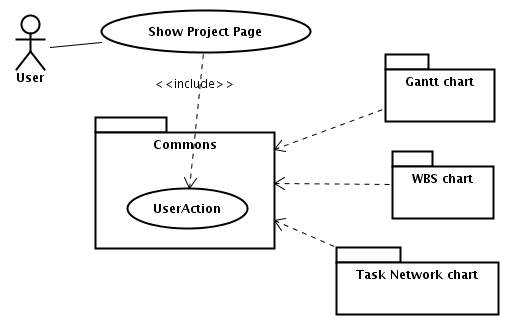
\includegraphics[width=0.8\textwidth]{EntireSystem.png} 
\caption{Entire system UML diagram}
\label{fig:entireSystemDiagram}
\end{figure}

\chapter{Commons}
Per questo pacchetto di use case non riportiamo il diagramma UML in quanto gli
use cases che vengono descritti non hanno relazione tra loro, e il diagramma
risulterebbe non molto significativo in quanto composto solo da pallogrammi
indipendenti tra loro.
\section{Make Dependencies}
\label{seq:makeDependencies}
\subsection{Basic course}
Si assume che l'insieme di \emph{TaskBox} sia gi\`a costruito.\\\\
Il client richiede di rappresentare graficamente le
\emph{Finish-ToStartDependency} relative all'insieme di \emph{TaskBox} gi\`a
costruite.

Il sistema esegue questi passi:
\begin{enumerate}
  \item costruisce un insieme $Dep$ di coppie del tipo $(a,b)$, con $a,b \in
  $\emph{TaskBox}, tale che $(a,b) \in Dep \Leftrightarrow b$ non pu\`o
  iniziare finch\`e $a$ non \`e stata completata.
  \item per ogni coppia $(a,b) \in Dep$ costruisci una linea
  spezzata cdns.
\end{enumerate}

\subsection{Alternative course}
\begin{description}
\item[not well formed project] Se la struttura al albero WBS del progetto non
\`e ben formata allora si deve cercare di dare la migliore euristica possibile
per la rappresentazione delle dipendenze.

\end{description}
\section{Make NodeTaskbox}
\label{seq:makeNodeTaskbox}
\subsection{Basic course}
Il client prende un reference al \emph{WBSChartGenerator} e domanda di creare la
rappresentazione grafica di un \emph{Task}.

Il sistema esegue questi passi:
\begin{enumerate}
  \item recupera il \emph{Task} da rappresentare.
  \item costruisce la rappresentazione grafica, il \emph{NodeTaskbox}
    in base alla scelta \emph{WBSTreeSpecification}. Il \emph{NodeTaskbox} \`e
    una composizione di \emph{Strip}. Il sistema costruisce una
    biezione tra \emph{BoxedStrip} e le scelte presenti in 
    \emph{UserOptionsChoice} in questo modo:
    \begin{itemize}
      % task name
      \item se \emph{UserOptionsChoice} contiene
      \emph{TaskNameOption}, allora costruisce una
      \emph{Strip} contenente il nome del \emph{Task} cdns.
      
      % resources
   	  \item se \emph{UserOptionsChoice} contiene \emph{ResourcesDetailsOption},
    	allora sul margine destro della \emph{GanttTaskBox} appendi la stringa
    	contenente la lista delle risorse cdns.
    	
    	Altrimenti appendi sul margine destro l'effort cdns.
      
      % planned time frame
      \item	se \emph{UserOptionsChoice} contiene \emph{PlannedTimeFrameOption} 
     allora costruisce due \emph{Strip} adiacenti contenenti rispettivamente le
     date di inizio e fine \emph{Task} cdns.
    	
	  % actual time frame
    	\item se \emph{UserOptionsChoice} contiene \emph{ActualTimeFrameOption}
    	allora costruisce due \emph{Strip} adiacenti contenenti rispettivamente 
    	le date di inizio e fine \emph{Task} reali cdns.
    	
		% planned data
    	\item se \emph{UserOptionsChoice} contiene \emph{PlannedDataOption} allora
    	costruisce tre \emph{Strip} adiacenti contenenti rispettivamente la durata
    	pianificata, lo sforzo complessivo pianificato, il costo
    	pianificato del \emph{Task} cdns.
    	
    	%actual data
    	\item se \emph{UserOptionsChoice} contiene \emph{ActualDataOption} allora
    	costruisce tre \emph{Strip} adiacenti contenenti rispettivamente la durata
    	“dall’inizio ad oggi”, lo sforzo complessivo “ad oggi” effettuato, il
    	costo complessivo “ad oggi” del \emph{Task} cdns.
    	
    	% completition bar
		\item se \emph{UserOptionsChoice} contiene \emph{CompletitionBarOption}
		allora costruisce la barra di completamento del \emph{Task} cdns.
		
		\item to complete with the missing options
		
    \end{itemize}
\end{enumerate}

\subsection{Alternative course}
\begin{description}
  \item[troncamento del nome del \emph{Task}] se la stringa scritta supera la
  dimensione fissata nel documento di specifica, allora il sistema la tronca
  cdns.


\end{description}

\section{Show UserOptions}
\label{seq:showUserOptions}
\subsection{Basic course}
Il client digita l'URL della \emph{ProjectPage}\footnote{TODO:definire
ProjectPage nel documento dei Mockup}. 

Il sistema invia in risposta la pagina richiesta con i tre tab relativi ai
\emph{Chart} descritti nel documento \textbf{Domain Model}. 

Il client fa click sul tab relativo al \emph{Chart} che vuole visualizzare.

Il sistema costruisce il contenuto del tab inserendo una sequenza di
\emph{UserOption}. 

Il client esegue la sua selezione delle informazioni che
vuole visualizzare nel \emph{Chart} e clicca su un oggetto\footnote{come posso
speficare questo oggetto?} per domandare la generazione del \emph{Chart}.

Il sistema esegue questi passi:
\begin{enumerate}
  \item costruisce \emph{UserOptionsChoice} in base alle opzioni selezionate
  dal client.
  \item recupera i \emph{Task} da includere nel \emph{Chart}.
  \item esegue la generazione\footnote{dire che la generazione astrae sui
  formati: la richiesta potrebbe essere o la visualizzazione della gif nel
  browser come attualmente fa mango, altrimenti la richiesta di generazione
  pdf. Inserire questo paragrafo come un description sotto il punto a cui
  appartiene questa nota.}
\end{enumerate}

\subsection{Alternative course}
\begin{description}
\item[Nessuna \emph{UserOption} selezionata] Il client invia un request con 
selezione delle \emph{UserOption} vuota. Quindi il sistema genera il
\emph{Chart} con delle \emph{UserOption} di default\footnote{dedicare un
paragrafo in un qualche documento per definire quali sono le opzioni di
default per ciascun chart.}.
\end{description}

\chapter{Gantt chart}
\section*{Overall UML diagram}
\begin{figure}[h!] \centering
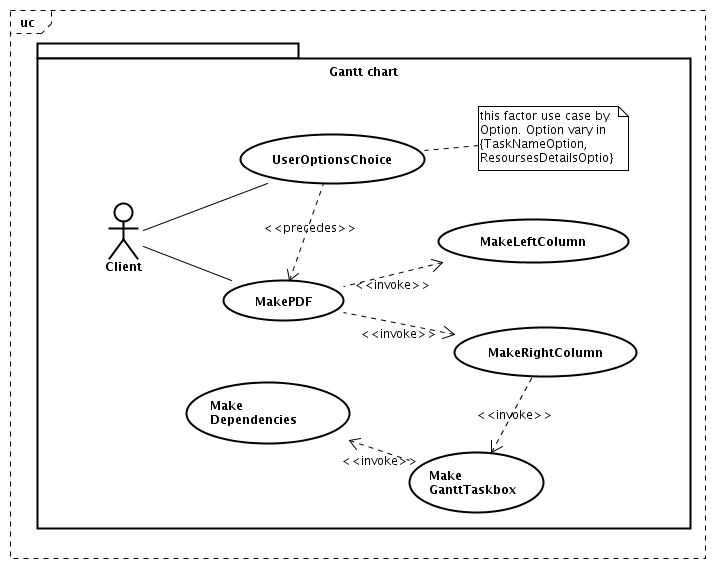
\includegraphics[width=0.8\textwidth]{Gantt/img/GanttChart.png} 
\caption{Gantt UML diagram}
\label{fig:ganttDiagram}
\end{figure}

\section{Make Left Column}
\label{seq:GanttMakeLeftColumn}
\subsection{Basic course}
Il client prende un reference al GanttChartGenerator e domanda la funzionalit\'a
per creare la colonna di sinistra del diagramma. \\
Il sistema costruisce una colonna di larghezza di dimensione \emph{fissa}.
Guarda se in UserOptionChoises \`e presente l'opzione TaskNameOption:
\begin{itemize}
  \item se \'e presente allora calcola la larghezza
\begin{displaymath}
	width_{nor}=lenght(max\lbrace id | \forall task: id =
WBS\_identifier(task) \rbrace) 
\end{displaymath}
dove la funzione $WBS\_identifier$ restituisce il WBS identifier relativo al 
parametro $task$ del dominio.

Poi $\forall task$ scrive $WBS\_identifier(task)$, un task per ogni riga.

\item altrimenti calcola
\begin{eqnarray}
width_{opt}=lenght(max\lbrace ::(id, task\_name) | \forall task: \\ id =
WBS\_identifier(task), \\ task\_name = Get\_TaskName(task)
\rbrace)
\end{eqnarray}
dove l'operatore $::$ concatena le stringhe passate come parametro, e
l'operatore \\$Get\_TaskName$ restituisce il nome del parametro
task.

Poi $\forall task$ scrive $::(WBS\_identifier(task), Get\_TaskName(task)$, un
task per ogni riga.
\end{itemize}

\subsection{Alternative course}
\begin{description}
\item[troncamento delle resourses] se $width_{opt} >
\frac{width_{diagram}}{6}$, con $width_{diagram}$ uguale alla larghezza totale
del diagramma, allora sia 
\begin{equation}cutted = cut(::(WBS\_identifier(task),
Get\_TaskName(task))\end{equation} 
la funzione $cut$ cancella caratteri in coda alla stringa in ingresso e
restituisce $cutted$, contenente i caratteri non cancellati, in modo che $cutted
= \frac{width_{diagram}}{6}-3$. \\ Il sistema scrive 
\begin{equation} 
::(cut(::(WBS\_identifier(task), Get\_TaskName(task)), ''\ldots'')
\end{equation}
\item[troncamento del WBS identifier] se avessi un identifier troppo lungo
dovrei fare lo stesso??
\end{description}
\section{Make GanttTaskbox}
\label{seq:makeGanttTaskbox}
\subsection{Basic course}
Il client prende un reference al GanttChartGenerator e domanda di creare la
rappresentazione grafica di un \emph{Task}. 

Il sistema esegue questi passi:
\begin{enumerate}
  \item recupera il \emph{Task} da rappresentare
  \item costruisce la rappresentazione grafica, il \emph{GanttTaskBox}
    in base alla scelta \emph{WBSTreeSpecification}.
  \item \`E possibile codificare delle informazioni aggiuntive:
    \begin{itemize}
   	  \item se \emph{UserOptionChoice} contiene \emph{ResourcesDetailsOption},
    	allora sul margine destro della \emph{GanttTaskBox} appendi la stringa
    	contenente la lista delle risorse cdns.
    	
    	Altrimenti appendi sul margine destro l'effort cdns.
    \end{itemize}
    
\end{enumerate}

\subsection{Alternative course}
\begin{description}
\item[troncamento delle resourses] se le informazioni testuali aggiuntive
superano la dimensione definita nel documento di specifica, allora si troncano
cdns.

\end{description}
\section{Make Right Column}
\label{seq:GanttRightRepresentation}
\subsection{Basic course}
Il client prende un reference al GanttChartGenerator e domanda di creare la
colonna di destra del diagramma. 

Il sistema esegue questi passi:
\begin{enumerate}
  \item costruisce una colonna di larghezza di dimensione \emph{fissa} che
  viene calcolata cdns.
  \item Il sistema effettua una ricerca per calcolare l'insieme dei \emph{Task}
  necessari da rappresentare nella colonna.
  \item Per ogni \emph{Task} trovato:
  \begin{itemize}
    \item invoca lo use case \ref{seq:makeGanttTaskbox}
    
    \item si posiziona il \emph{GanttTaskBox} creato nella giusta posizione
    temporale in base alla scelta \emph{TimeGrainOption}.
  \end{itemize}
  \item se \emph{UserOptionsChoice} contiene \emph{ShowDependencies} allora per
  ogni \emph{TaskBox} rappresentata, invoca lo use case 
  \ref{seq:makeDependencies}
\end{enumerate}

\subsection{Alternative course}
\begin{description}
\item[troncamento delle resourses] se le informazioni testuali aggiuntive
superano la dimensione definita nel documento di specifica, allora si troncano
cdns.

\end{description}
\section{Make PDF}
\label{seq:GanttMakePDF}

\subsection{Basic course}
Il client entra nella pagina relativa al diagramma Gantt e clicca sulla 
funzionalit\`a ''Make PDF''. Il sistema costruisce un oggetto in questo modo:
\begin{itemize}
  \item invoca lo use case \ref{seq:GanttMakeLeftColumn} per creare la
  colonna a sinistra.
  \item invoca lo use case \ref{seq:GanttRightRepresentation} per creare
  la rappresentazione nel tempo (colonna destra del diagramma).
\end{itemize}
Il sistema invio la pagina di risposta al client, aggiungendo accanto ai
pulsanti di reporting una icona per permettere il download del file generato.  

\subsection{Alternative course}
\begin{description}
\item[nessuna]
\end{description}



\chapter{WBS chart}
\section*{Overall UML diagram}
\begin{figure}[h!] \centering
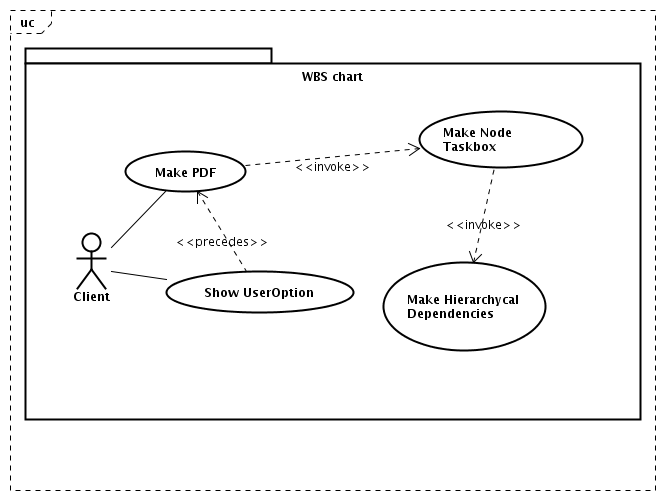
\includegraphics[width=0.8\textwidth]{WBS/WBSChart.png}
\caption{WBS UML diagram}
\label{fig:WBSdiagram}
\end{figure}

\section{Make Hierarchycal Dependencies}
\label{seq:makeHierarchycalDependencies}
\subsection{Basic course}
Il client richiede la funzionalità di rappresentazione della relazione 
gerarchica di un task.

Il sistema esegue questi passi:
\begin{enumerate}
  \item in base alle informazioni in \emph{WBSTreeSpecification}, recupera i
  figli del task (non l’intera discendenza, solo quelli di livello successivo) e
  li dispone graficamente al di sotto di esso.
  \item La distanze fra livelli e tra taskbox appartenenti allo stesso
  livello rispettano queste regole:
  \begin{itemize}
    \item la distanza \emph{inter-Taskbox} fra coppie di
    \emph{Taskbox} adiacenti, rappresentati sullo stesso livello, deve essere
    equa ed uguale per ogni coppia (questa regola si ripete in modo iterativo
    per ogni coppia appartenente ad un livello $l$)
	\item la distanza \emph{inter-Level} fra coppie di livelli contenenti le 
	rappresentazioni dei task padre e i suoi figli deve essere equa e uguale
	per ogni coppia di livelli (questa regola si applica ricorsivamente al livello
	dei figli, nel caso che almeno un figlio sia composto da subtask)
  \end{itemize} 
  
  \item Il sistema collega il task ai suoi figli con linee spezzate cdns.
\end{enumerate}

\subsection{Alternative course}
\begin{description}
\item[WBSExplosionLevel = 0] se il livello di visualizzazione della WBSStructure
richiesto si limita alla root, crea il solo un \emph{NodeTaskbox} rappresentante
l’intero progetto.
\end{description}


\section{Make PDF}
\label{seq:GanttMakePDF}

\subsection{Basic course}
Il client entra nella pagina relativa al diagramma Gantt e clicca sulla 
funzionalit\`a ''Make PDF''. Il sistema costruisce un oggetto in questo modo:
\begin{itemize}
  \item invoca lo use case \ref{seq:GanttMakeLeftColumn} per creare la
  colonna a sinistra.
  \item invoca lo use case \ref{seq:GanttRightRepresentation} per creare
  la rappresentazione nel tempo (colonna destra del diagramma).
\end{itemize}
Il sistema invio la pagina di risposta al client, aggiungendo accanto ai
pulsanti di reporting una icona per permettere il download del file generato.  

\subsection{Alternative course}
\begin{description}
\item[nessuna]
\end{description}



\end{document}